\documentclass[11pt]{article}
\usepackage[a4paper,margin=1in]{geometry}
\usepackage[utf8]{inputenc}
\usepackage[T1]{fontenc}
\usepackage{amsmath,amssymb}
\usepackage{graphicx}
\usepackage{booktabs}
\usepackage{hyperref}

\graphicspath{{images/}}

\title{\textbf{Directed Emergence of Network Structure Under an Energy Budget}}
\author{Vasili Gavrilov\thanks{Independent researcher. Physics and computer
science by education; a professional software engineer with a background in
numerical optimization and machine learning, including a genetic-algorithm
optimizer built for industrial use in 2002. Reference implementation:
\url{https://github.com/Anode1/SMBPANN}, 2001--2015--2026.}}
\date{2026}

\begin{document}
\maketitle

\begin{abstract}
A network's structure should \emph{emerge}, not be designed, but from what, and how much of it? We grow a
network's topology from an \textbf{exhaustive, fully-connected seed under an evolutionary energy budget}
that pays for every connection, and ask honestly which pieces of convolution fall out. Sparse
task-relevant connectivity emerges cleanly; weight sharing is \emph{adopted} when translation invariance
rewards it; and a compact aligned local filter emerges too, but only once mutation acts on the shared
feature the way real genetics does, not on a single edge. On top of the priors a ConvNet hardwires
(locality and translatability), the free dimensions then organize to the task: compact fields, depth that
matches the required receptive field, channels that match the number of distinct operations, up to a
capacity limit four interventions fail to move.

\medskip\noindent\textbf{What is new:}
-the sharing/energy \emph{decoupling}, why a compact filter cannot emerge under per-connection pruning yet
does once mutation acts on the shared feature, which restores the missing energy gradient;
-that \emph{directed} evolutionary search beats random sampling of structures, and the advantage
\emph{holds across scale} once its search budget scales with the problem, reversing the near-null our
companion crossover study found on a real benchmark;
-the honest energy-emergence map from an exhaustive seed, its negatives kept.
The rest reproduces textbook inductive-bias facts (weight sharing is data-efficient, receptive
field~$\approx$~depth), verified with a fair baseline rather than claimed as new. Every number regenerates
from one \texttt{make}; the dead-ends are kept.
\end{abstract}

\section{Introduction}

This project has a long fuse. A 1997 thesis argued only that heuristics, inductive bias built into the
architecture by hand, are a \emph{necessity} for a trainable, generalizing network~\cite{bpfnn97}. The
ambition to instead let the architecture \emph{emerge} from a genetic-algorithm search, not be
hand-designed, in the best case rediscovering the convolutional receptive field (Figure~\ref{fig:main}),
came in 2002, after the author had worked with genetic algorithms in industry; the project was created in
2015 and first implemented only now, in pure C. A companion study on that side of the idea, \emph{searching} whole
topologies and cells, reached a firmly negative conclusion: on the real NAS-Bench-101 cell space, no
crossover meaningfully beats random search, and structure-aware operators do worse than a structure-blind
one, because good cells are common and the gap to the optimum sits inside the benchmark's own training
noise. Searching for structure did not beat random.

This paper comes at the same ambition from the opposite end. Instead of searching for the architecture,
we \emph{grow} one: start from an exhaustive, fully-connected seed, put a cost on every connection, and
watch which parts of convolution survive the squeeze. The question is not ``can a search find a good
architecture'' but ``what structure emerges, on its own, under an energy budget, and what refuses to.''

\begin{figure}[t]
\centering
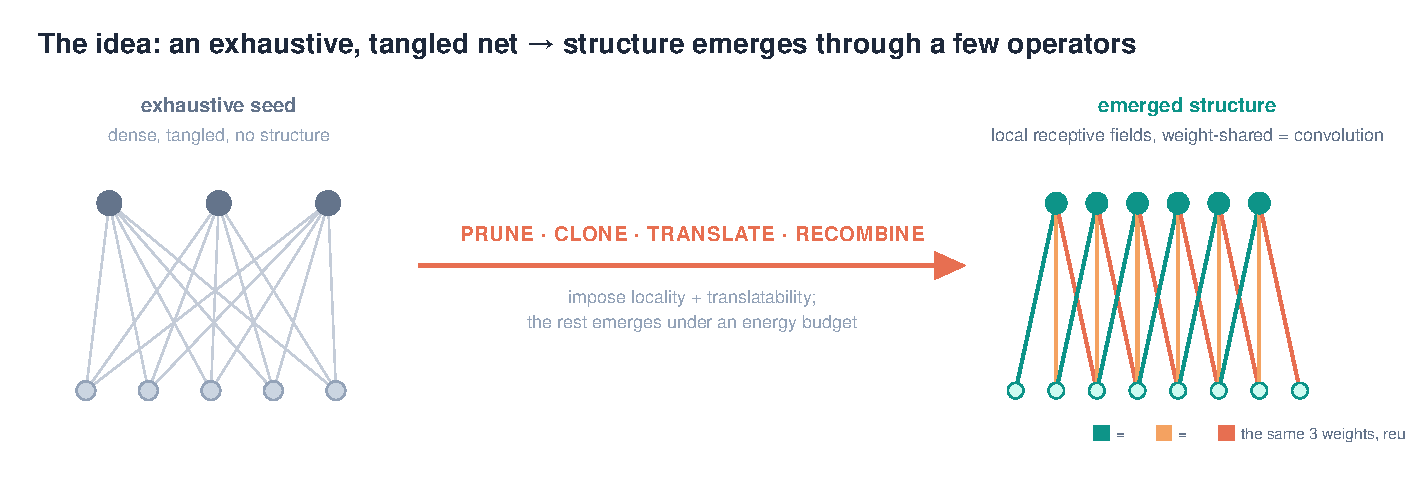
\includegraphics[width=0.95\textwidth]{fig_main_idea.pdf}
\caption{The idea. An exhaustive, tangled network becomes an ordered convolution through a few
structural operators. We impose the domain's real symmetries (locality, translatability) and let
prune, clone, translate, and recombine assemble and refine the rest.}
\label{fig:main}
\end{figure}

\paragraph{Contribution, stated honestly.} The genuinely new part is the map: the specific
\emph{evolutionary energy-emergence from an exhaustive seed}, and its boundaries. We are not aware of a
prior result showing this together with the mechanism the compact filter needs in order to emerge at all
(grouped mutation on the shared feature, not the single edge). This is distinct from gradient pruning (Optimal Brain Damage; the Lottery
Ticket), from DARTS' gradient-relaxed supernet, and from NEAT's grow-from-minimal, which augment rather
than prune. Much of the rest, weight sharing is data-efficient; receptive field $\approx$ depth,
reproduces known inductive-bias facts, which we verify carefully rather than claim as new. The value is
the honest characterization, the negatives, and the full reproducibility; not the underlying mechanisms.

\paragraph{Method in one paragraph.} A one-hidden-layer network whose connectivity is a binary mask is
evolved by a genetic algorithm from an all-ones (dense) seed. Fitness is validation accuracy on a scarce
training set; the objective is to minimize energy (the number of connections, or free parameters) subject
to accuracy $\geq$ target. Mutation is mostly-prune, rarely-grow, an annealing schedule, in which a
prune is a downhill move in energy and a rare added connection is an uphill thermal fluctuation. All
numbers below are means over independent seeds; each experiment is a self-contained C99 probe.

\section{What emerges, and what does not}

\subsection{Pruning: feature selection emerges; convolution does not}

Under an energy budget the search prunes a dense connectivity mask to a sparse one, and on a task whose
label depends on a few specific inputs it lands \textbf{90\%} of the surviving connections on the
task-relevant inputs (chance $0.33$, no-selection drift $0.34$). Feature selection, discovering
\emph{which} inputs matter, emerges cleanly (Figure~\ref{fig:prune}). What does \emph{not} emerge is
the aligned local receptive field: at comparable density the surviving connections are no more in-window
than chance, so the search finds \emph{a} sparse subnetwork, not \emph{the} convolutional one, exactly
the outcome of the pruning literature (sparse subnetworks, not convolutions).

\begin{figure}[t]
\centering
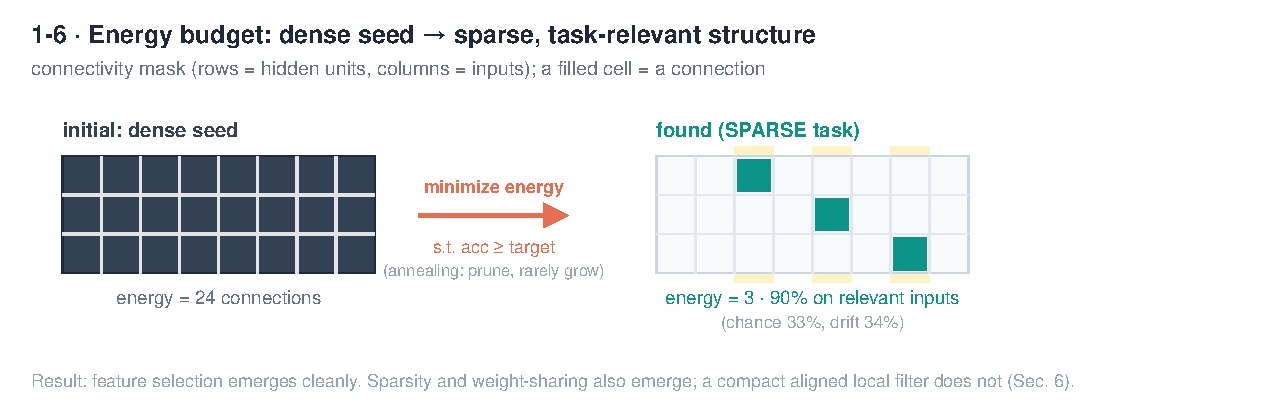
\includegraphics[width=0.9\textwidth]{fig1_pruning.pdf}
\caption{Sections 2--3. An energy budget prunes a dense connectivity seed to a sparse mask whose
surviving connections land on the task-relevant inputs. Feature selection and sparsity emerge; the
compact aligned filter needs mutation on the shared feature to emerge (Sec.~2.3).}
\label{fig:prune}
\end{figure}

\subsection{Imposing locality: a compact filter emerges, sharing is adopted}

Locality is not something to wait out; a bounded receptive field is a law of the problem (information is
local), and every ConvNet imposes it. When we impose only that, each hidden unit sees a
\emph{contiguous} window, a compact local field falls right out: the width anneals to a mean of
$\approx K$ (the kernel size), the compact filter the energy budget alone could not produce. A
weight-tying gene (tie weights by within-window offset, i.e.\ translation invariance) is \emph{adopted}
by $0.89$ of the population; but its accuracy benefit is within noise, and the shared arm stays wider,
because shared energy charges only the maximum width, so the mean has no gradient. The pieces of
convolution keep emerging separately; the clean compact \emph{shared} whole does not dominate.

\subsection{The compact filter, and the mutation that finds it}

There is a subtlety in what ``an energy budget'' means here, and it is, we think, the paper's one real
insight. Once weights are shared, removing a single connection no longer reduces the parameter count,
that offset is still used by other positions, so a mutation acting on one edge has no energy gradient to
tighten the kernel. The right unit of mutation is not the edge but the shared feature.

\paragraph{The compact filter does emerge, under the right mutation.} Biological mutation is global, not
local: a change to a gene acts on every instance of the mechanism it builds (all the ``similar blocks and
duplicated edges''), not on one edge. So for a weight-shared filter the natural unit of mutation is the
shared \emph{offset}, all the connections that reuse that weight; flipping a whole offset removes all its
duplicated edges in one move and reduces the parameter count, which restores the energy gradient a
single-connection edit cannot give. Under this grouped mutation the kernel contracts: the surviving tap
count falls to $2.6$ (near $K=3$) over 16 seeds, and a width penalty sharpens it to contiguity $0.80$ on
the generative offsets. It is not a perfect $K=3$ kernel (span $\approx 4$), and the offset genome makes
the connectivity translation-invariant by construction, but the compact filter largely emerges once
mutation acts on the shared mechanism, as real genetics does.

\paragraph{And it emerges from either direction.} For completeness: run the same energy GA under grouped
mutation from a \emph{minimal} seed and grow up (a NEAT-style direction), and it reaches an essentially
identical kernel to the dense seed pruned down (taps $3.5$ vs $3.8$, contiguity $0.77$ vs $0.80$,
24 seeds). The emergence does not depend on the starting point: grow-from-minimal and prune-from-dense
converge on the same structure.

\subsection{Directed search vs.\ random, and the budget it needs}

Does the \emph{directed} energy search do real work, or would random sampling of the same structures find
the compact filter just as well? The question is sharp because on a real benchmark our companion crossover
study found evolution barely edges random, inside the noise. \textbf{Method.} At a \emph{matched
evaluation budget}, we run the grouped-mutation GA against random offset masks (drawn across densities,
kept by the same objective) over 50 \emph{paired} seeds (same task per seed) at five input sizes $N$, once
at a fixed budget and once at a budget that scales with $N$ (Figure~\ref{fig:directed}, Table~\ref{tab:directed}).

\begin{table}[t]
\centering\small
\begin{tabular}{@{}rccccc@{}}
\toprule
 & \multicolumn{2}{c}{contiguity} & \multicolumn{2}{c}{paired GA${-}$random gap} & \\
\cmidrule(lr){2-3}\cmidrule(lr){4-5}
$N$ & GA & random & fixed budget & scaled budget & win/tie/loss \\
\midrule
12 & 0.73 & 0.71 & $+0.02{\pm}0.03$ & $+0.02{\pm}0.03$ & 12/29/9 \\
16 & 0.68 & 0.61 & $+0.07{\pm}0.04$ & $+0.06{\pm}0.04$ & 23/11/16 \\
20 & 0.67 & 0.46 & $+0.21{\pm}0.04$ & $+0.22{\pm}0.03$ & 37/6/7 \\
24 & 0.56 & 0.41 & $+0.15{\pm}0.04$ & $+0.17{\pm}0.03$ & 37/2/11 \\
28 & 0.52 & 0.45 & $+0.07{\pm}0.04$ & $\mathbf{+0.15{\pm}0.04}$ & 33/1/16 \\
\bottomrule
\end{tabular}
\caption{Directed GA vs random at matched evaluations, 50 paired seeds. Contiguity and win/tie/loss are
at fixed budget; the last two columns give the paired advantage under a fixed budget and under one scaled
to $N$. The fixed-budget gap erodes at $N{=}28$; with budget scaled to the problem it holds.}
\label{tab:directed}
\end{table}

\begin{figure}[t]
\centering
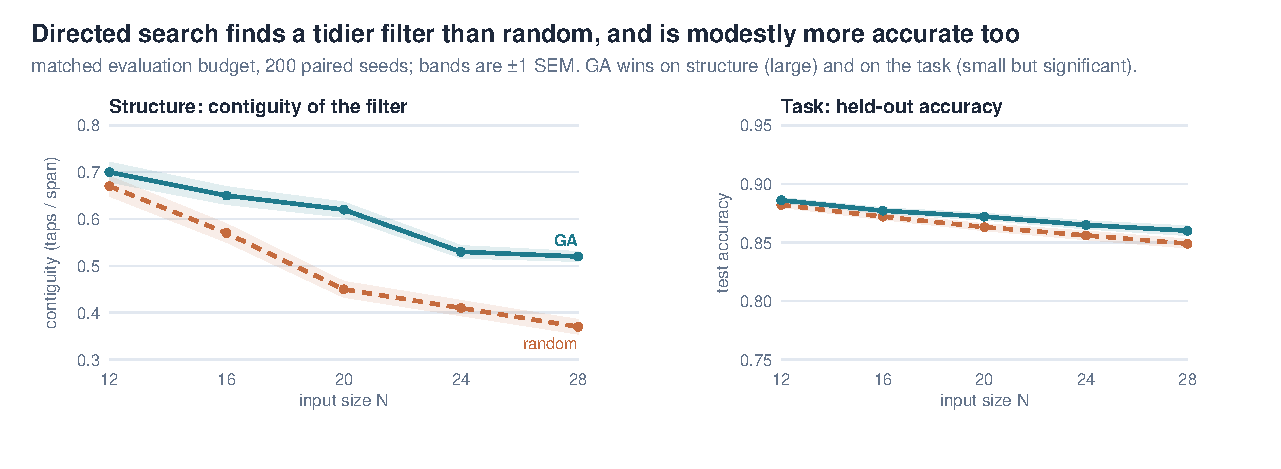
\includegraphics[width=0.95\textwidth]{fig6_directed.pdf}
\caption{Directed search vs random, across scale. \emph{Left:} the paired GA${-}$random contiguity gap; the
fixed-budget curve falls at $N{=}28$ (the GA is starved as the space grows to $2^{54}$ masks), the
scaled-budget curve holds. \emph{Right:} the GA's own contiguity recovers with budget while random stays
flat. 50 paired seeds, matched evaluations per arm.}
\label{fig:directed}
\end{figure}

\textbf{Result.} Directed search wins, and the win \emph{holds across scale} once its budget is fair. At
trivial size the two tie ($N{=}12$, gap $+0.02$): the filter is easy, random finds it too. The gap is
decisive by $N{=}20$ (paired $+0.21{\pm}0.04$, 37 wins to 7 losses of 50). Under a fixed budget it appears
to fall back at $N{=}28$ ($+0.07$), but that is the GA being starved, not random catching up: scale the
budget with $N$ and the $N{=}28$ gap doubles to $+0.15{\pm}0.04$ while the GA's contiguity recovers
($0.52{\to}0.59$) and random stays flat ($\approx 0.44$). So directed search holds a clear advantage over
random across scale ($\approx +0.15$ to $+0.22$, all ${\geq}3.7$ SEM from $N{=}20$ to $28$) \emph{provided
its budget scales with the problem}; the advantage is sustained, not monotonically growing. This reverses
the crossover null: there evolution only tied random inside the benchmark's noise; here, under an energy
budget, it beats random outright.

\subsection{Emergent depth matches the required receptive field}

Impose the feed-forward composition rule too, stack one reused block type, and the one dimension
left free, the depth, emerges to fit the task. On a task that fires only when two spikes are exactly
distance $s$ apart (so a unit must see both at once, needing receptive field $\geq s{+}1$, i.e.\ depth
$\geq s/2$), accuracy sits at chance until the stack is deep enough to span the pair, then lifts off at
depth $\approx s/2$; larger $s$ selects a deeper stack (Figure~\ref{fig:depth}). This is the clearest
positive of the emergence side: given the necessary priors, the free dimension organizes itself to the
task.

\begin{figure}[t]
\centering
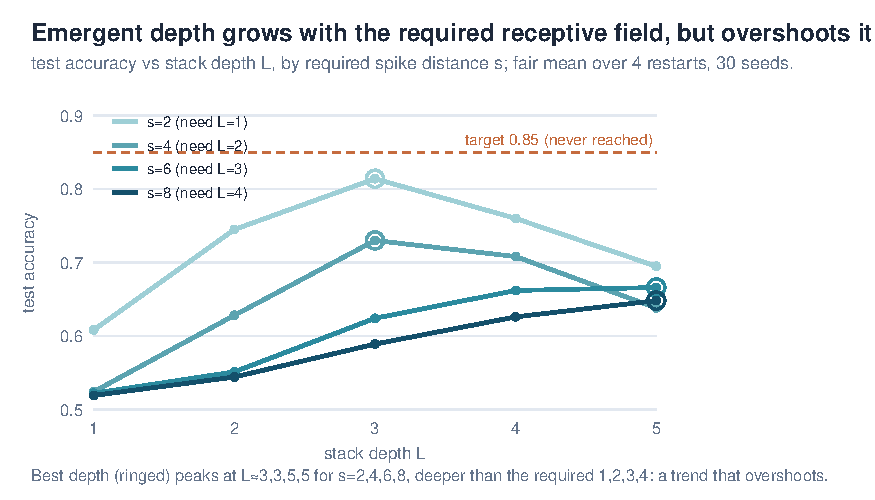
\includegraphics[width=0.9\textwidth]{fig3_depth.pdf}
\caption{Emergent depth matches the required receptive field. Accuracy is at chance until the stack is
deep enough for its receptive field to span the spike pair, then lifts off at depth $\approx s/2$.}
\label{fig:depth}
\end{figure}

\begin{figure}[t]
\centering
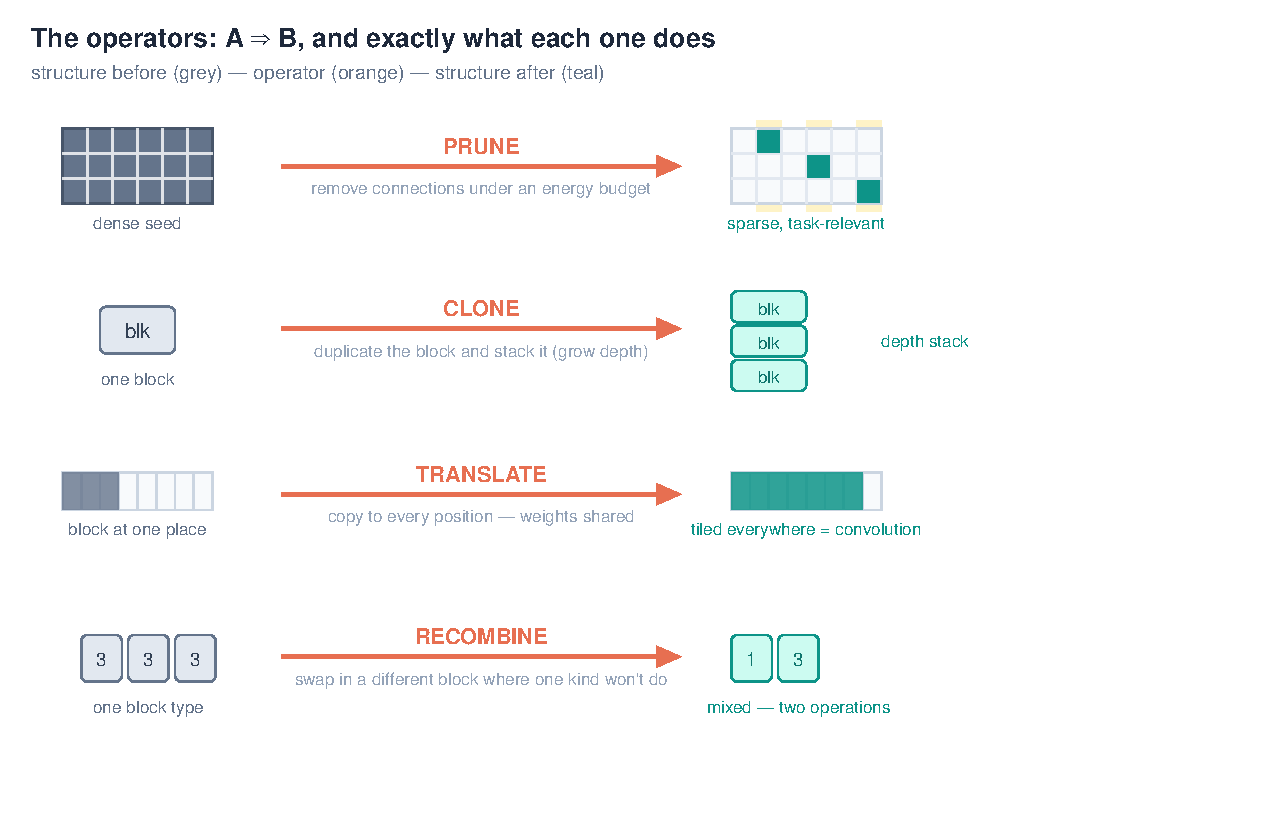
\includegraphics[width=0.9\textwidth]{fig_operators.pdf}
\caption{The four structural operators as $A \to B$, each with its exact action. Prune (remove
connections under an energy budget), clone (duplicate and stack, for depth), translate (copy to every
position with shared weights, a convolution), recombine (swap in a different block where one kind will
not do). Each maps to a biological analog: pruning, gene/segment duplication, transposition/serial
homology, sexual recombination.}
\label{fig:ops}
\end{figure}

\section{The operators: reuse, recombination, translation}

\subsection{Reuse beats a free search at equal compute}

Composing blocks explodes combinatorially, so we adopt the heuristic LeCun did: reuse one block type,
stacked, and search only the depth. At \emph{equal compute}, a free heterogeneous search (a GA over
arbitrary block sequences, using a dilated-conv library) never solves more reliably or at lower energy
than simply enumerating uniform reused blocks; on the harder tasks reuse is strictly better. Block
diversity buys nothing but a larger search, the reuse heuristic is the tractable near-optimum, which
is the user's intuition (``the combinations explode, so reuse the same block'') made quantitative. This
mirrors cell-based NAS (ENAS, DARTS), which search one cell and stack it.

\subsection{Recombination is required when a task needs two different operations}

Reuse breaks exactly where the biology predicts. On a task that needs a fine local motif
$(+,-,+)$ at adjacent positions (visible only to a dilation-1 block) \emph{and} a far spike at distance
$s$ (reached cheaply only by a dilation-3 block), no single reused block serves both roles: a uniform
dilation-3 stack is blind to the fine motif (solving 0/8), a uniform dilation-1 stack cannot afford the
reach. Recombination, a GA over mixed block sequences, solves 8/8 at about half the energy, and its
solutions are literal two-operation mixes such as $[1,3]$: one fine block, one coarse-reach block
(Figure~\ref{fig:reuse}). Clone when scaling a working module; recombine only when you need a new kind of
part, runners when the structure repeats, seeds when it must change.

\begin{figure}[t]
\centering
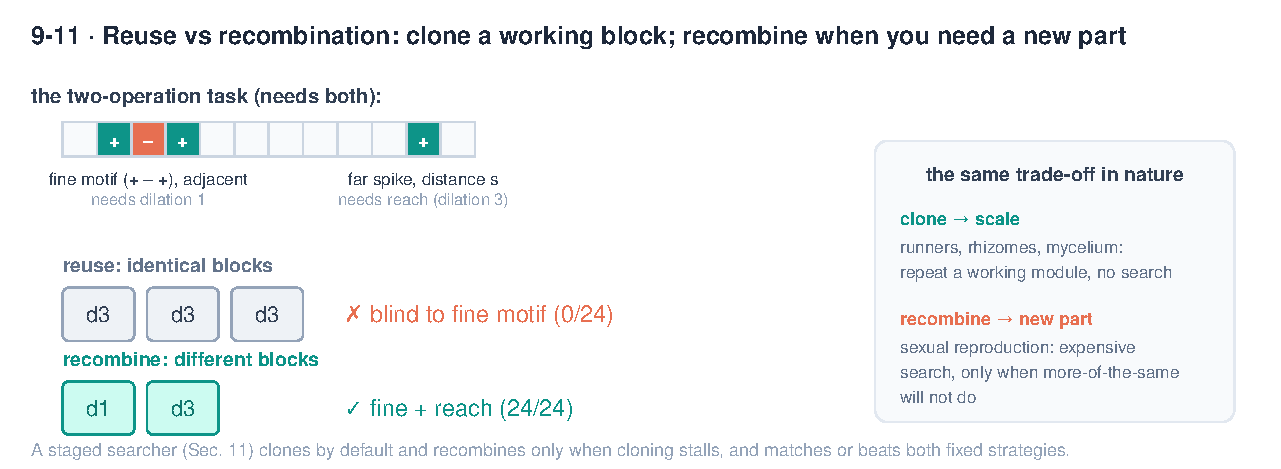
\includegraphics[width=0.95\textwidth]{fig4_reuse.pdf}
\caption{Reuse vs recombination, and the clone/recombine trade-off nature also makes. One reused block
suffices for repetitive structure; a task needing two different operations forces recombination of
different blocks.}
\label{fig:reuse}
\end{figure}

\subsection{Translation: weight sharing is data-efficient (a reproduction, fairly done)}

The third operator, translation, replicating one working detector across positions with shared
weights (transposition, serial homology, cortical-map tiling), is exactly convolution's tiling,
reached by replication. On a translation-invariant motif task we compare a weight-shared filter (3
weights) against a locally-connected baseline (one filter per position). Table~\ref{tab:translate} gives
the fair result (mean over restarts, $\pm 1$ SD over $40$ seeds): the shared filter wins at every train
size, most so when data is scarcest (gap $+0.24$ at 16 examples, $+0.14$ at 128 as the baseline slowly
catches up). This is the textbook argument for weight sharing (one filter learns the motif from every
position's examples while each independent filter starves), here quantified with a fair estimator. It is
a phenomenon of weight \emph{sharing}, not of architecture search: the two arms are weight-tied vs untied,
both trained by plain SGD.

\begin{table}[t]
\centering
\begin{tabular}{lccc}
\toprule
train size & weight-shared & locally-connected & gap \\
\midrule
16 & $0.820 \pm 0.122$ & $0.581 \pm 0.065$ & $+0.239$ \\
32 & $0.838 \pm 0.094$ & $0.615 \pm 0.071$ & $+0.224$ \\
64 & $0.866 \pm 0.082$ & $0.672 \pm 0.076$ & $+0.195$ \\
128 & $0.867 \pm 0.081$ & $0.724 \pm 0.086$ & $+0.143$ \\
\bottomrule
\end{tabular}
\caption{Weight sharing is data-efficient. Shared filter (3 weights) vs locally-connected (42 weights),
by training-set size. The advantage is largest at the scarcest data.}
\label{tab:translate}
\end{table}

\subsection{The advantage widens with input size, then saturates}

Sweeping input size $N$ (so the number of positions to cover grows), the shared arm stays flat at
$\approx 0.94$ (always 3 weights, size-independent) while the locally-connected baseline falls to chance
($0.52$) and bloats to $378$ weights, because each per-position filter starves on the
$\approx n_{\mathrm{tr}}/P$ examples that land there (Figure~\ref{fig:scale}, $250$ seeds). The gap is
4--6$\times$ the SD, so the effect is significant. Honestly stated it \emph{widens then saturates}: most
growth is $N{=}16\to32$, after which the baseline has already hit the chance floor. The effect survives
even a fully-trained, oracle-supervised locally-connected baseline (which we hand the motif locations):
the shared arm still wins $+0.14$ at $N{=}16$ up to $+0.38$ at $N{=}128$, so it is not an artifact of the
baseline's training rule.

\begin{figure}[t]
\centering
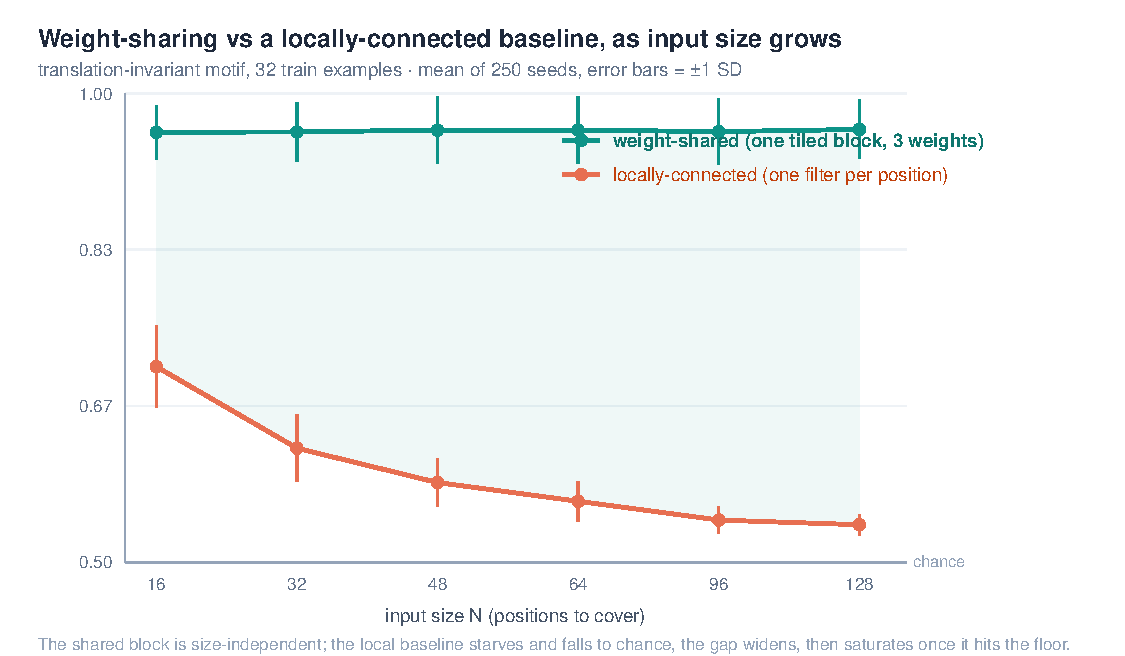
\includegraphics[width=0.85\textwidth]{fig_scale_chart.pdf}
\caption{The weight-sharing advantage as input size grows (mean of 250 seeds, error bars $\pm 1$ SD).
The shared block is size-independent; the locally-connected baseline starves and falls to chance. The
gap widens, then saturates once the baseline hits the floor.}
\label{fig:scale}
\end{figure}

\section{An honest boundary in 2-D}

In two dimensions ``two different operations'' means two feature \emph{channels}, a horizontal and a
vertical filter, since one channel is one orientation. A task requiring both orientations present
caps a single channel near $0.75$ (the analytic ceiling a lone orientation detector can reach), and
accuracy rises with channels ($0.69 \to 0.77 \to 0.86 \to 0.89$ over $C{=}1{\ldots}4$, $24$ seeds): a
gradual rise, not a sharp $C{=}2$ jump, but the load-bearing fact, one channel is not enough for two
operations, is significant. The tidy generalization ``channel count = operation count,'' however,
\textbf{fails}: growing channels to solve a $K$-operation task gives selected $C^\ast \approx 1.2, 3.2,
5.0$ for $K{=}1,2,3$, so $K{=}2$ already overshoots and $K{=}3$ breaks, sub-target at every channel
count ($C{=}5$: $0.79$), only 2 of 24 seeds solving.

This K=3 wall is genuine, not under-training. Four interventions fail to move it: more channels, a
nonlinear (MLP) readout, competition (lateral inhibition, the mechanism that self-organizes cortical
orientation columns), and, with a budget caveat, a deeper extractor. An independent heavy-compute
rerun ($2.5\times$ epochs, $2\times$ signal) leaves $K{=}3$ sub-target at every channel count, confirming
the wall is structural for the channel axis. Per-channel detection error compounds multiplicatively
($0.95^3 \approx 0.86$, at the target edge), and no cheap refinement moves a multiplicative wall; real
vision clears such tasks with scale (depth, normalization, residuals, vast data), not one clever
pressure. We report this boundary plainly: it is more honest than stopping at small $K$ where the
staircase still looked clean.

\section{Related work, and how we differ}

The closest neighbors, and the honest distinction: \textbf{DARTS} starts from an exhaustive supernet and
prunes to a final architecture, closest in spirit, but via continuous gradient relaxation over
predefined operations, not an energy GA, and it never asks whether convolution emerges. \textbf{Optimal
Brain Damage} and the \textbf{Lottery Ticket Hypothesis} prune dense to sparse, but by gradient
magnitude, and find sparse subnetworks, not convolutions. \textbf{NEAT}, \textbf{HyperNEAT}, and
Cellular Encoding evolve topology but \emph{grow from a minimal seed}, the opposite direction to pruning
from exhaustive. \textbf{Cell-based NAS} (ENAS, regularized evolution) reuses one cell and stacks it,
which our reuse observations echo. We claim the honest characterization of what an evolutionary energy
budget does and does not produce, and the negatives, not the underlying mechanisms, which are known.

\medskip\noindent Two framings place this experiment in a longer line. The view of network topology as
problem-specific inductive bias that must be engineered by hand goes back decades~\cite{bpfnn97}; here we
ask the complementary question, whether that structure can instead \emph{emerge} from the energy budget
rather than be built in.\footnote{The broader claim that such emergence is substrate-independent is
argued informally in a companion essay~\cite{emergence_sub}.} Viewed more broadly, the energy budget is a
description-length pressure: the emergent weight-shared filter is a compressor whose inductive bias,
locality and sharing, matches the task's translation symmetry, an instance of the evolutionary-search
route to compressor discovery set out in~\cite{compressors}.

\section{Limitations}

The tasks are small synthetic constructions built so the intended structure is optimal; they demonstrate
what emerges under an energy budget on a task shaped like convolution, and do not by themselves
generalize to real data. The reuse/scale results are weight-\emph{sharing} data efficiency, not
architecture search; we relabel them accordingly. The full developmental pipeline chaining all four
operators on a genuinely compositional task, and a real dataset, are the natural next steps; the K=3
``wall'' is a capacity limit of \emph{this} shallow conv $+$ max-pool setup, and whether a properly
trained deeper net clears it is open. The honest home of this work is an explainer or a negative-results
workshop, not a novelty venue.

\section{Conclusion}

Impose the domain's real symmetries; let a few biological operators assemble the rest. Under an energy
budget on an exhaustive seed, sparsity and feature selection emerge and weight sharing is adopted, and a
compact convolution emerges too, but only once mutation acts on the shared feature rather than the single
edge, for a decoupling reason we can state in a line. On top of imposed priors,
depth emerges to match the receptive field, reuse beats a free search at equal compute, recombination is
required only when a task needs a genuinely different operation, and weight-shared tiling is
data-efficient at a degree that grows with scale then saturates. Where it runs out, a three-way
conjunction unmoved by four fixes, we say so. The contribution is the honest map, the negatives, and
the reproducibility; every number regenerates from one command.

\begin{thebibliography}{9}
\bibitem{obd} Y.~LeCun, J.~S. Denker, S.~A. Solla. Optimal Brain Damage. \emph{NeurIPS} 1990.
\bibitem{lecun89} Y.~LeCun et al. Backpropagation Applied to Handwritten Zip Code Recognition.
 \emph{Neural Computation} 1(4), 1989.
\bibitem{lottery} J.~Frankle, M.~Carbin. The Lottery Ticket Hypothesis. \emph{ICLR} 2019.
\bibitem{darts} H.~Liu, K.~Simonyan, Y.~Yang. DARTS: Differentiable Architecture Search. \emph{ICLR} 2019.
\bibitem{enas} H.~Pham, M.~Guan, B.~Zoph, Q.~Le, J.~Dean. Efficient Neural Architecture Search via
 Parameter Sharing. \emph{ICML} 2018.
\bibitem{neat} K.~O. Stanley, R.~Miikkulainen. Evolving Neural Networks through Augmenting Topologies.
 \emph{Evolutionary Computation} 10(2), 2002.
\bibitem{amoeba} E.~Real, A.~Aggarwal, Y.~Huang, Q.~V. Le. Regularized Evolution for Image Classifier
 Architecture Search. \emph{AAAI} 2019.
\bibitem{kirkpatrick} S.~Kirkpatrick, C.~D. Gelatt, M.~P. Vecchi. Optimization by Simulated Annealing.
 \emph{Science} 220, 1983.
\bibitem{repo} V.~Gavrilov. SMBPANN reference implementation, 2001--2015--2026.
 \url{https://github.com/Anode1/SMBPANN}.
\bibitem{compressors} V.~Gavrilov. Intelligence Is the Discovery of Compressors. 2026.
 \url{https://doi.org/10.5281/zenodo.20440111}.
\bibitem{bpfnn97} V.~Gavrilov. Backpropagation Feed-Forward Neural Networks. Seminar thesis, Open
 University of Israel, 1997 (digitized 2026). \url{https://doi.org/10.5281/zenodo.20450526}.
\bibitem{emergence_sub} V.~Gavrilov. Emergence Does Not Care About Substrate. Companion essay, 2026.
 \url{https://gavr144.substack.com/p/emergence-does-not-care-about-substrate}.
\end{thebibliography}

\end{document}
